% Para utilizar este template siga o tutorial disponível em http://www.biblioteca.ufc.br/wp-content/uploads/2015/09/tutorial-sharelatex.pdf

%%%%%%%%%%%%%%%%%%%%%%%%%%%%%%%%%%%%%%%%%%%%%%%%%%%%%%%
%% Você deve criar uma conta no Overleaf. Depois,    %%
%% vá nas opções no canto esquerdo superior da tela  %%
%% e clique em "Copiar Projeto". Dê um novo nome pa- %%
%% ra o projeto.                                     %%
%%                                                   %%
%% Os principais desenvolvedores deste template são: %%
%%                                                   %%
%%            Ednardo Moreira Rodrigues              %%
%%       (Doutor em Engenharia Elétrica - UFC)       %%
%%(Coord. do Grupo de Astronomia da Seara da Ciência)%%
%%                      &                            %%
%%            Alan Batista de Oliveira               %%
%%           (Engenheiro Eletricista - UFC)          %%
%%                                                   %%
%% Consultoria Bibliotecária                         %%
%%                                                   %%
%%  Versão 2016 - ShareLaTeX:                        %% 
%%                                                   %%
%% - Francisco Edvander Pires Santos;                %%
%% - Juliana Soares Lima;                            %%
%% - Izabel Lima dos Santos;                         %%
%% - Kalline Yasmin Soares Feitosa;                  %%
%% - Eliene Maria Vieira de Moura.                   %%
%% ------------------------------------------------- %% 
%%  Versão 2019,2020 - Overleaf:                     %%
%%                                                   %%
%%  Biblioteca de Ciências Humanas:                  %%
%% - Francisco Edvander Pires Santos;                %%
%% - Juliana Soares Lima;                            %%
%% - Eliene Maria Vieira de Moura;                   %%
%% - Edmundo Moreira de Sousa Filho.                 %%
%%                                                   %%
%% Biblioteca da FEAAC:                              %%
%% - Izabel Lima dos Santos;                         %%
%% - Kalline Yasmin Soares Feitosa;                  %%
%% - Kleber Lima dos Santos.                         %%
%%                                                   %%
%%  Biblioteca do Curso de Física:                   %%
%% - Aline Rodrigues de Lima Mendes;                 %%
%% - Maria de Jesus Silva dos Santos.                %%
%%                                                   %%
%%  Biblioteca Central do Campus do Pici:            %%
%% - Raquel da Silva Nascimento.                     %%
%% - Felipe Ferreira da Silva                        %%
%%  Versão 2019,2020 - Overleaf:                     %%
%%  ------------------------------------------------ %%
%%  Versão de 2022 - Overleaf                        %%
%%                                                   %%
%%   a) Felipe Ferreira da Silva                        %%
%%   b) Ednardo Moreira Rodrigues                       %%
%%   c) Comissão de Normalização do Sistema de          %%
%%      Bibliotecas da UFC                              %%
%%                                                   %%
%% Colaboradores                                     %%
%%                                                   %%
%% -Andrei Bosco Bezerra Torres                      %% 
%% (Professor - Sistemas e Mídias Digitais -         %%
%% Instituto Universidade Virtual - UFC)             %%
%% Tiago Alves Lima                                  %% 
%% (Aluno de Mestrado em Eng. Elétrica)              %%
%%                                                   %%
%% Grande parte do trabalho foi adaptado do template %%
%% da UECE elaborado por:                            %%
%% Thiago Nascimento  (UECE)                         %%
%% Project available on:                             %%
%% https://github.com/thiagodnf/uecetex2             %%
%%                                                   %%
%% "Dúvidas, esclarecimentos ou sugestões podem ser  %%
%% enviadas para o seguinte e-mail:                  %%
%%                                                   %%
%%             bu@ufc.br               %%
%%                                                   %%
%% As últimas atualizações estão descritas no inicio %%
%% do arquivo "README.md".                           %%
%%                                                   %%
%%%%%%%%%%%%%%%%%%%%%%%%%%%%%%%%%%%%%%%%%%%%%%%%%%%%%%%

\documentclass[        
    a4paper,          % Tamanho da folha A4
    12pt,             % Tamanho da fonte 12pt
    chapter=TITLE,    % Todos os capitulos devem ter caixa alta
    section=Title,    % Todas as secoes devem ter caixa alta somente na primeira letra
    subsection=Title, % Todas as subsecoes devem ter caixa alta somente na primeira letra
    oneside,          % Usada para impressao em apenas uma face do papel
    english,          % Hifenizacoes em ingles
    spanish,          % Hifenizacoes em espanhol
    brazil,           % Ultimo idioma eh o idioma padrao do documento
    fleqn             % Comente esta linha se quiser centralizar as equacoes. Comente também a linha 65 abaixo
]{lib/abntex2}

% Para utilizar este template siga o tutorial disponível em http://www.biblioteca.ufc.br/wp-content/uploads/2015/09/tutorial-sharelatex.pdf

%%%%%%%%%%%%%%%%%%%%%%%%%%%%%%%%%%%%%%%%%%%%%%%%%%%%%%%
%% Você deve criar uma conta no Overleaf. Depois,    %%
%% vá nas opções no canto esquerdo superior da tela  %%
%% e clique em "Copiar Projeto". Dê um novo nome pa- %%
%% ra o projeto.                                     %%
%%                                                   %%
%% Os principais desenvolvedores deste template são: %%
%%                                                   %%
%%            Ednardo Moreira Rodrigues              %%
%%       (Doutor em Engenharia Elétrica - UFC)       %%
%%(Coord. do Grupo de Astronomia da Seara da Ciência)%%
%%                      &                            %%
%%            Alan Batista de Oliveira               %%
%%           (Engenheiro Eletricista - UFC)          %%
%%                                                   %%
%% Consultoria Bibliotecária                         %%
%%                                                   %%
%%  Versão 2016 - ShareLaTeX:                        %% 
%%                                                   %%
%% - Francisco Edvander Pires Santos;                %%
%% - Juliana Soares Lima;                            %%
%% - Izabel Lima dos Santos;                         %%
%% - Kalline Yasmin Soares Feitosa;                  %%
%% - Eliene Maria Vieira de Moura.                   %%
%%                                                   %% 
%%  Versão 2019 - Overleaf:                          %%
%%                                                   %%
%%  Biblioteca de Ciências Humanas:                  %%
%% - Francisco Edvander Pires Santos;                %%
%% - Juliana Soares Lima;                            %%
%% - Eliene Maria Vieira de Moura;                   %%
%% - Edmundo Moreira de Sousa Filho.                 %%
%%                                                   %%
%% Biblioteca da FEAAC:                              %%
%% - Izabel Lima dos Santos;                         %%
%% - Kalline Yasmin Soares Feitosa;                  %%
%% - Kleber Lima dos Santos.                         %%
%%                                                   %%
%%  Biblioteca do Curso de Física:                   %%
%% - Aline Rodrigues de Lima Mendes;                 %%
%% - Maria de Jesus Silva dos Santos.                %%
%%                                                   %%
%%  Biblioteca Central do Campus do Pici:            %%
%% - Raquel da Silva Nascimento.                     %%
%% - Felipe Ferreira da Silva                        %%
%%                                                   %%
%% Colaboradores                                     %%
%%                                                   %%
%% -Andrei Bosco Bezerra Torres                      %% 
%% (Professor - Sistemas e Mídias Digitais -         %%
%% Instituto Universidade Virtual - UFC)             %%
%% Tiago Alves Lima                                  %% 
%% (Aluno de Mestrado em Eng. Elétrica)              %%
%%                                                   %%
%% Grande parte do trabalho foi adaptado do template %%
%% da UECE elaborado por:                            %%
%% Thiago Nascimento  (UECE)                         %%
%% Project available on:                             %%
%% https://github.com/thiagodnf/uecetex2             %%
%%                                                   %%
%% "Dúvidas, esclarecimentos ou sugestões podem ser  %%
%% enviadas para o seguinte e-mail:                  %%
%%                                                   %%
%%             atendimentobch@ufc.br                 %%
%%                                                   %%
%% As últimas atualizações estão descritas no inicio %%
%% do arquivo "README.md".                           %%
%%                                                   %%
%%%%%%%%%%%%%%%%%%%%%%%%%%%%%%%%%%%%%%%%%%%%%%%%%%%%%%%

% Importações de pacotes
\usepackage[utf8]{inputenc}                         % Acentuação direta
\usepackage[T1]{fontenc}                            % Codificação da fonte em 8 bits
\usepackage{graphicx}                               % Inserir figuras
\usepackage{amsfonts, amssymb, amsmath}             % Fonte e símbolos matemáticos
\usepackage{booktabs}                               % Comandos para tabelas
\usepackage{verbatim}                               % Texto é interpretado como escrito no documento
\usepackage{multirow, array}                        % Múltiplas linhas e colunas em tabelas
\usepackage{indentfirst}                            % Endenta o primeiro parágrafo de cada seção.
\usepackage{listings}                               % Utilizar codigo fonte no documento
\usepackage{xcolor}
\usepackage{microtype}                              % Para melhorias de justificação?
\usepackage[portuguese,ruled,lined]{algorithm2e}    % Escrever algoritmos
\usepackage{algorithmic}                            % Criar Algoritmos  
%\usepackage{float}                                 % Utilizado para criação de floats
\usepackage{amsgen}
\usepackage{lipsum}                                 % Usar a simulação de texto Lorem Ipsum
%\usepackage{titlesec}                              % Permite alterar os títulos do documento
\usepackage{tocloft}                                % Permite alterar a formatação do Sumário
\usepackage{etoolbox}                               % Usado para alterar a fonte da Section no Sumário
\usepackage[nogroupskip,nonumberlist]{glossaries}   % Permite fazer o glossario. A apcao "sort=use" faz com que as siglas aparecam na lista conformse sao usadas no texto.

\usepackage[format=plain,justification=justified,skip=0pt,singlelinecheck = false,labelsep=colon]{caption}            % Altera o comportamento da tag caption. Algumas opcoes do caption so podem ser alternada no arquivo "antex2.cls, linhas 334 a 348.

\usepackage[alf, abnt-emphasize=bf, recuo=0cm, abnt-etal-cite=2, abnt-etal-list=0, abnt-etal-text=it]{lib/ufcTexcite}  % Citações padrão UFC/ABNT NBR 6023 de 2018
%\usepackage[bottom]{footmisc}                      % Mantém as notas de rodapé sempre na mesma posição
%\usepackage{times}                                 % Usa a fonte Times
%%%%%%%%%%%%%%%%%%% AVISO %%%%%%%%%%%%%%%%%%%%%%%%%%%%%%%%%%%%%%%%
%descomente as duas linhas abaixo para alterar o texto de Times New Roman para Arial:

%\usepackage{helvet}
%\renewcommand{\familydefault}{\sfdefault}  % Usa a fonte Arial              
%%%%%%%%%%%%%%%%%%%%%%%%%%%%%%%%%%%%%%%%%%%%%%%%%%%%%%%%%%%%%%%%%%

\usepackage{mathptmx}         % Usa a fonte Times New Roman			%\usepackage{lmodern}         % Usa a fonte Latin Modern
%\usepackage{subfig}          % Posicionamento de figuras
%\usepackage{scalefnt}        % Permite redimensionar tamanho da fonte
%\usepackage{color, colortbl} % Comandos de cores
%\usepackage{lscape}          % Permite páginas em modo "paisagem"
%\usepackage{ae, aecompl}     % Fontes de alta qualidade
%\usepackage{picinpar}        % Dispor imagens em parágrafos
%\usepackage{latexsym}        % Símbolos matemáticos
%\usepackage{upgreek}         % Fonte letras gregas
\usepackage{appendix}         % Gerar o apendice no final do documento
\usepackage{paracol}          % Criar paragrafos sem identacao
\usepackage{lib/ufcTex}	      % Biblioteca com as normas da UFC para trabalhos academicos
\usepackage{pdfpages}         % Incluir pdf no documento
\usepackage{amsmath}          % Usar equacoes matematicas

\makeglossaries % Organiza e gera a lista de abreviaturas, simbolos e glossario
\makeindex      % Gera o Indice do documento         

\renewcommand{\labelitemi}{\textendash} %Altera os marcadores de itemize para 





\setlength{\mathindent}{0pt} %Complementa o alinhamento de equações para totalmente a esquerda.

%%%%%%%%%%%%%%%%%%%%%%%%%%%%%%%%%%%%%%%%%%%%%%%%%%%%%
%%                     ATENCAO                     %%
%%%%%%%%%%%%%%%%%%%%%%%%%%%%%%%%%%%%%%%%%%%%%%%%%%%%%
%  Qual e o nivel do trabalho academico que voce esta 
% escrevendo? Retire o simbolo "%" apenas de um dos 
% quatro topicos abaixo refente ao nível do seu traba
% -lho.

%\trabalhoacademico{tccgraduacao}
%\trabalhoacademico{tccespecializacao}
\trabalhoacademico{dissertacao}
%\trabalhoacademico{tese}

%%%%%%%%%%%%%%%%%%%%%%%%%%%%%%%%%%%%%%%%%%%%%%%%%%%%%

% Define se o trabalho e uma qualificacao
% Coloque 'nao' para versao final do trabalho

\ehqualificacao{nao}

% Remove as bordas vermelhas e verdes do PDF gerado
% Coloque 'sim' pare remover

\removerbordasdohyperlink{sim} 

% Adiciona a cor Azul a todos os hyperlinks

\cordohyperlink{nao}

%%%%%%%%%%%%%%%%%%%%%%%%%%%%%%%%%%%%%%%%%%%%%%%%%%%%%
%%         Informacao sobre a instituicao          %%
%%%%%%%%%%%%%%%%%%%%%%%%%%%%%%%%%%%%%%%%%%%%%%%%%%%%%

\ies{Universidade Federal do Ceará}
\iessigla{UFC}
\centro{Centro de Xxxxxxxx}
\departamento{Departamento de Xxxxxxxxx}

%%%%%%%%%%%%%%%%%%%%%%%%%%%%%%%%%%%%%%%%%%%%%%%%%%%%%
%%        Informacao para TCC de Graduacao         %%
%%%%%%%%%%%%%%%%%%%%%%%%%%%%%%%%%%%%%%%%%%%%%%%%%%%%%

\graduacaoem{Engenharia Xxxxxxx}
\habilitacao{bacharel} % Ou licenciado(a)

% AVISO: Caso necessario alterar o texto de apresenta-
% cao da Especializacao, ir a pasta "lib", arquivo 
% "ufctex.sty" na linha 502.


%%%%%%%%%%%%%%%%%%%%%%%%%%%%%%%%%%%%%%%%%%%%%%%%%%%%%
%%     Informacao para TCC de Especializacao       %%
%%%%%%%%%%%%%%%%%%%%%%%%%%%%%%%%%%%%%%%%%%%%%%%%%%%%%

\especializacaoem{Yyyyyyyyy}

% AVISO: Caso necessario alterar o texto de apresenta-
% cao da Especializacao, ir a pasta "lib", arquivo 
% "ufctex.sty" na linha 507.

%%%%%%%%%%%%%%%%%%%%%%%%%%%%%%%%%%%%%%%%%%%%%%%%%%%%%
%%         Informacao para Dissertacao             %%
%%%%%%%%%%%%%%%%%%%%%%%%%%%%%%%%%%%%%%%%%%%%%%%%%%%%%

\programamestrado{Programa de Pós-Graduação em Xxxxxxx}
\nomedomestrado{Mestrado Acadêmico em Xxxxxxx}
\mestreem{Engenharia Xxxxxx}
\areadeconcentracaomestrado{Engenharia Xxxxxx}

% AVISO: Caso necessario alterar o texto de apresenta-
% cao da dissertacao, ir a pasta "lib", arquivo 
% "ufctex.sty" na linha 511.

%%%%%%%%%%%%%%%%%%%%%%%%%%%%%%%%%%%%%%%%%%%%%%%%%%%%%
%%               Informação para Tese              %%
%%%%%%%%%%%%%%%%%%%%%%%%%%%%%%%%%%%%%%%%%%%%%%%%%%%%%

\programadoutorado{Programa de Pós-Graduação em Xxxxxx}
\nomedodoutorado{Doutorado em Xxxxxxx}
\doutorem{Engenharia Xxxxxx}
\areadeconcentracaodoutorado{Engenharia Xxxxxxx}

% AVISO: Caso necessario alterar o texto de apresenta-
% cao da tese, ir a pasta "lib", arquivo "ufctex.sty" 
% na linha 515.

%%%%%%%%%%%%%%%%%%%%%%%%%%%%%%%%%%%%%%%%%%%%%%%%%%%%%
%%      Informacoes relacionadas ao trabalho       %%
%%%%%%%%%%%%%%%%%%%%%%%%%%%%%%%%%%%%%%%%%%%%%%%%%%%%%

\autor{Nome Sobrenome}
\titulo{Título do Trabalho: subtítulo (se houver)}
\data{2022}
\local{Fortaleza}

% Exemplo: \dataaprovacao{01 de Janeiro de 2012}
\dataaprovacao{xx/xx/xxxx.}

%%%%%%%%%%%%%%%%%%%%%%%%%%%%%%%%%%%%%%%%%%%%%%%%%%%%%
%%           Informação sobre o Orientador         %%
%%%%%%%%%%%%%%%%%%%%%%%%%%%%%%%%%%%%%%%%%%%%%%%%%%%%%

\orientador{Prof. Dr. Xxxxxxx Xxxxxx Xxxxxxx}
\orientadories{Universidade Federal do Ceará (UFC)}
\orientadorcentro{Centro de Ciências e Tecnologia (CCT)}
\orientadorfeminino{nao} % Coloque 'sim' se for do sexo feminino

%%%%%%%%%%%%%%%%%%%%%%%%%%%%%%%%%%%%%%%%%%%%%%%%%%%%%
%%          Informação sobre o Coorientador        %%
%%%%%%%%%%%%%%%%%%%%%%%%%%%%%%%%%%%%%%%%%%%%%%%%%%%%%

% Deixe o nome do coorientador em branco para remover do documento

\coorientador{Prof. Dr. Xxxxxx (Se houver)}
\coorientadories{Universidade Coorientador (SIGLA)}
\coorientadorcentro{Centro do Coorientador (SIGLA)}
\coorientadorfeminino{nao} % Coloque 'sim' se for do sexo feminino

%%%%%%%%%%%%%%%%%%%%%%%%%%%%%%%%%%%%%%%%%%%%%%%%%%%%%
%%              Informação sobre a banca           %%
%%%%%%%%%%%%%%%%%%%%%%%%%%%%%%%%%%%%%%%%%%%%%%%%%%%%%

% Atenção! Deixe em branco o nome do membro da banca para remover da folha de aprovacao

% Exemplo de uso:
% \membrodabancadois{Prof. Dr. Fulano de Tal}
% \membrodabancadoisies{Universidade Federal do Ceará - UFC}


\membrodabancadois{Prof. Dr. Xxxxxxx Xxxxxx Xxxxxxx}
\membrodabancadoiscentro{Faculdade de Filosofia Dom Aureliano Matos (FAFIDAM)}
\membrodabancadoisies{Universidade do Membro da Banca três (SIGLA)}
\membrodabancatres{Prof. Dr. Xxxxxxx Xxxxxx Xxxxxxx}
\membrodabancatrescentro{Centro de Ciências e Tecnologia (CCT)}
\membrodabancatresies{Universidade do Membro da Banca quatro (SIGLA)}
\membrodabancaquatro{Prof. Dr. Xxxxxxx Xxxxxx Xxxxxxx}
\membrodabancaquatrocentro{Centro de Ciências e Tecnologia (CCT)}
\membrodabancaquatroies{Universidade do Membro da Banca cinco (SIGLA)}
\membrodabancacinco{Prof. Dr. Xxxxxxx Xxxxxx Xxxxxxx}
\membrodabancacincocentro{Teste}
\membrodabancacincoies{Universidade do Membro da Banca seis (SIGLA)}
\membrodabancaseis{Prof. Dr. Xxxxxxx Xxxxxx Xxxxxxx}
\membrodabancaseiscentro{}
\membrodabancaseisies{Universidade do Membro da Banca sete (SIGLA)}

\begin{document}	

	% Elementos pré-textuais
	%\imprimircapa
	%\imprimirfolhaderosto{}
	%\imprimirfichacatalografica{1-pre-textuais/ficha-catalografica}
	%\imprimirerrata{elementos-pre-textuais/errata}
	%\imprimirfolhadeaprovacao
	%\imprimirdedicatoria{1-pre-textuais/dedicatoria}
	%\imprimiragradecimentos{1-pre-textuais/agradecimentos}
	%\imprimirepigrafe{1-pre-textuais/epigrafe}
	%\imprimirresumo{1-pre-textuais/resumo}
	%\imprimirabstract{1-pre-textuais/abstract}
	%\renewcommand*\listfigurename{Lista de Figuras} %Se você comentar esta linha o título da lista fica: LISTA DE ILUSTRAÇÕES
	%\imprimirlistadeilustracoes
	%\imprimirlistadetabelas
	%\imprimirlistadequadros
	%\imprimirlistadealgoritmos
	%\imprimirlistadecodigosfonte
	%\imprimirlistadeabreviaturasesiglas
	%\imprimirlistadesimbolos{1-pre-textuais/lista-de-simbolos}   
	%\imprimirsumario
	
	%\setcounter{table}{0}% Deixe este comando antes da primeira tabela.
	
	%Elementos textuais
	\textual
	\chapter{Introdução}
\label{cap:introducao}

O mercado de artes digitais sempre se mostrou um lugar difícil para os artistas. Em um mercado onde a garantia de valores como legitimidade e unicidade é fundamental, a demasiada facilidade de reprodução fornecida por ferramentas digitais torna a garantia desses valores uma tarefa ingrata. O colecionismo, atividade comum a quem costuma adquirir obras de arte, é praticamente inexistente em contextos digitais. A unicidade gera uma exclusividade que é muito particular a esse segmento, diferenciando-o de outras obras criativas, como a música, cujo mercado encontrou seu caminho através dos streamings. No entanto, a música sempre teve grande apelo reprodutivo, através das rádios e mídias fabricadas em larga escala, logo, a capacidade de reprodução fornecida por meios digitais não representava uma barreira como representa para obras de arte. 

Essas dificuldades fazem com que boa parte dos artistas opte por não comercializar suas obras por meios digitais, dando preferência a impressos. Ainda assim, o risco da reprodução não consentida persiste, dada a popularidade de meios de cópia disponíveis. Nesse sentido, as NFTs surgem como uma interessante alternativa. Sigla para Non-Fungible Tokens, as NFTs pertencem ao contexto das Blockchains, a base técnica por trás do funcionamento de criptomoedas como Bitcoin e Ethereum. Uma NFT nada mais é do que um Token cuja natureza é única, graças as suas propriedades que permitem sua distinção de um Token para outro. Eles podem representar qualquer tipo de item, desde um ingresso de um jogo de futebol a uma obra de arte, e graças as características das Blockchain, que incluem descentralização e protocolos de consenso, tornaram-se uma opção importante para publicação e venda de artefatos como obras de arte. 






Se no mercado de artes tradicionais é possível garantir essa 





Tokens não fungíveis. Essa é a tradução livre para Non-Fungible Tokens, palavras que juntas formam a sigla NFT. Ela ficou famosa nos últimos anos com o advento de seu uso, ligado ao contexto do mercado das artes digitais e tendo sido inclusive um dos assuntos mais buscados por brasileiros no Google em 2022 . Sua existência está ligada as Blockchains, tecnologia base para o funcionamento de criptomoedas como Bitcoin e Ethereum. Um Token não fungível é um token cuja natureza é única, ou seja, é possível diferencia-lo de um para outro graças as suas propriedades, diferente de Tokens convencionais. 


	\chapter{Fundamentação teórica}
\label{cap:fundamentacao-teorica}

\section{Non-Fungible Tokens}
\label{cap:non-fungible tokens}

Non-Fungible \textit{token}s, ou \textit{tokens} não fungíveis em tradução livre, são as palavras que compõem a sigla NFT. Ela ganhou popularidade nos últimos anos, tendo sido eleita a palavra do ano 2020 pelo dicionário Collins \footnote{Disponível em: <https://g1.globo.com/tecnologia/noticia/2021/11/24/nft-e-eleita-a-palavra-do-ano-2020-pelo-dicionario-collins.ghtml> Acesso em: 12 jan, 2023}, continuando popular em 2022, sendo destaque nas pesquisas realizadas por brasileiros no Google \footnote{Disponível em: <https://einvestidor.estadao.com.br/ultimas/nft-destaque-buscas-google-2022> Acesso em: 12 jan, 2023}. Essa popularidade se deve as movimentações de grandes cifras monetárias em torno de um novo tipo de item virtual que inundaram os noticiários e as redes sociais, especialmente com o envolvimento de pessoas famosas, a exemplo do atleta Neymar Jr, que na ocasião investiu cerca de 790 mil reais em um desses itens \cite{Andrade}. Esses itens virtuais nada mais eram que imagens, desenhos e fotografias, entre outros tipos de artefatos visuais, comercializados a partir de redes \textit{\textit{blockchain}} \footnote{conceito de \textit{blockchain} aqui}.

Em uma \textit{blockchain}, \textit{token}s são unidades de troca e podem assumir diversas representações, incluindo moedas, registros, identidades, entre outros \cite{Antonopoulos, Voshmgir}. Um \textit{token} não fungível é um tipo de \textit{token} cuja natureza é única, com propriedades variáveis capazes de diferenciar uns dos outros \cite{Voshmgir}. Segundo o Dicionário Priberam da Língua Portuguesa, o adjetivo "fungível" significa algo que se gasta após primeiro o uso, ou seja, que é descartável ou substituível, assim, a não-fungibilidade se refere a unicidade representada por esse tipo de \textit{token}, a sua exclusividade. Por serem propagados em redes \textit{blockchain}, os NFT trazem consigo as garantias desse tipo de rede, que consistem em mecanismos públicos e distribuídos de validação, propagação e comercialização desses ativos. Esse conjunto de fatores fez com que os NFT se tornassem um interessante meio para propagação de obras artísticas, embora não fiquem limitados a elas, conforme explica Voshmgir:

\begin{citacao}
	 Os NFT podem também representar identidades e certificados, tais como licenças, graus, chaves, passes, identidades, testamentos, direitos de voto, bilhetes, \textit{token}s de fidelização, direitos de autor, garantias, licenças de software, dados médicos, e certificados de qualquer tipo, tais como cadeias de fornecimento ou certificados de arte \cite{Voshmgir}
\end{citacao}

No entanto, é interessante notar como as possibilidades oferecidas pelos NFT resolvem em grande parte as dores dos artistas e outros profissionais que fornecem produtos cuja exclusividade é posta em cheque pela natureza intuitiva das mídias digitais. Conforme explica o fotógrafo Alex Montesso, "Um NFT é um certificado de propriedade de um ativo digital que não pode ser alterado ou falsificado", concluindo que "essa certificação garante a rastreabilidade e certifica a peça como autêntica" \cite{Montesso}. Para o escritor Logan Kugler, essa capacidade (de certificar uma propriedade digital) exclusiva era algo impensável até o surgimento dos NFT: 

\begin{citacao}
Essa dinâmica cria uma simples, mas poderosa forma de como trabalhar com artes digitais, tornando-as exclusivas. Uma vez cunhado na \textit{blockchain} Ethereum, o NFT é representado em um livro-razão público que não pode ser alterado. Ao possuir o \textit{token}, você prova ser dono da obra de arte. Não há nada que impeça sua visualização online, ou mesmo sua cópia e compartilhamento, mas sem a NFT, não é possível fingir a posse da obra de arte (...) \cite{Kugler}
\end{citacao}

Cunhar é o verbo que se refere a publicação de um NFT, ou seja, a sua inserção no livro-razão pertencente a uma \textit{blockchain}. Um livro-razão, também conhecido como \textit{ledger}, é um arquivo que mantém uma lista incremental de registos de transações, em blocos ligados criptograficamente, protegidos de adulteração e revisão. Em uma \textit{blockchain}, esse arquivo é mantido de forma distribuída, sendo público e auditável por todos os participantes da rede \cite{Voshmgir, Lyra}. É a essa estrutura que se deve a capacidade de um NFT em resguardar a exclusividade de uma obra, bem como prover garantias aos seus donos, sejam criadores ou colecionadores. Isso também garante a capacidade de transferir obras para outros indivíduos, permitindo a revenda desses itens.

Outra característica importante introduzida pelos NFT foi a capacidade de gerar escassez artificial em obras digitais de forma escalável e eficiente \cite{Kugler}. Um arquivo digital pode ser copiado infinitamente sem que perca suas características, algo que pode inviabilizar o controle de reprodução e, por consequência, a capacidade de garantir a autenticidade de uma obra. Para Guilherme Preger, os NFT vão num sentido contrário à da reprodutibilidade dos meios digitais, valorizando a autenticidade e a singularidade dessas obras \cite{Preger}. Ao cunhar um NFT, o artista pode definir uma quantidade limitada de itens referentes a uma determinada obra, garantindo que somente quem tiver posse desses \textit{token}s será um proprietário verdadeiro dessas obras. 

Transferir qualquer tipo de titularidade (ou posse) de artefatos digitais também é uma demanda de vários segmentos. Ao longo dos últimos anos, várias tentativas de controlar a distribuição de produtos como e-books e músicas por meios digitais sempre esbarraram em limitações de ordem técnica e ou mesmo de direitos básicos do consumidor, como revenda e até mesmo de empréstimo. O DRM\footnote{Mecanismo complexo de proteção baseado em inúmeras tecnologias com objetivo de vincular conteúdo específico a um determinado grupo de permissões de acesso e uso, em operação integrada a instrumentos de monitoramento e registro de consumo \cite{Vieira}}, a mais popular dessas tentativas, além de limitar o direito dos consumidores, privilegia plataformas (limitando a experiência e liberdade de uso) e sequer conseguem garantir os direitos dos autores, dadas as vulnerabilidades nesse sistema. Os NFT permitem operações de troca, revenda e até a possibilidade de presentear com esses itens digitais, desde que ambas as partes estejam em uma mesma \textit{blockchain}, o que não representa um grande problema, já que carteiras digitais \footnote{explicar o que é uma carteira digital} mais populares permitem a conexão com várias redes distintas. 

Originalmente, NFT estão disponíveis através da plataforma Ethereum, uma \textit{blockchain} de código aberto que executa programas chamados contratos inteligentes e permite que desenvolvedores criem variadas aplicações descentralizadas \cite{Antonopoulos}. Entre essas aplicações, estão outras criptomoedas e até o objeto deste trabalho, os NFT. Em uma \textit{blockchain}, um contrato inteligente, ou \textit{smart-contracts} é uma ferramenta de gestão de direitos que pode formalizar e executar acordos auto-executáveis entre participantes não confiáveis \cite{Voshmgir}. Por meio desses contratos, é possível embutir em um NFT um conjunto de regras nos termos de venda, que podem incluir inclusive o pagamento automático de royalties ao artista sempre que a obra mudar de mãos em uma ocasião de revenda, por exemplo \cite{Kugler}.














	%\chapter{Metodologia}
\label{chap:metodologia}

Texto texto texto texto texto texto texto texto texto texto texto texto texto texto texto texto texto texto texto texto texto texto texto texto texto texto texto texto texto texto texto texto texto texto texto texto texto texto texto texto texto texto texto texto texto texto texto texto texto texto texto texto texto texto texto texto texto texto texto texto texto texto texto texto texto texto texto texto texto.

Texto texto texto texto texto texto texto texto texto texto texto texto texto texto texto texto texto texto texto texto texto texto texto texto texto texto texto texto texto texto texto texto texto texto texto texto texto texto texto texto texto texto texto texto texto texto texto texto texto texto texto texto texto texto texto texto texto texto texto texto texto texto texto texto texto texto texto texto texto.

\section{Exemplo de alíneas}\label{sec:exemplo-de-algoritmos-e-figuras}

    Texto texto texto texto texto texto texto texto texto texto texto texto texto texto texto texto texto texto texto texto texto texto texto texto texto texto texto texto texto texto texto texto texto texto texto texto texto texto texto texto texto texto texto texto texto texto texto texto texto texto texto texto texto texto texto texto texto texto texto texto texto texto texto texto texto texto texto texto texto.

    %\begin{algorithm}[h!]
    %	\SetSpacedAlgorithm
    %	\caption{\label{exemplo-de-algoritmo}Como escrever algoritmos no \LaTeX2e}
    %	\Entrada{o proprio texto}
    %	\Saida{como escrever algoritmos com  Latex:}% \LaTeX2e }
    %	\Inicio{
    %		inicialização;
    %		\Repita{fim do texto}{
    %			leia o atual;
    %			\Se{entendeu}{
    %				vá para o proximo\;
    %				próximo se torna o atual;}
    %			\Senao{volte ao início da seção;}
    %		}
    %	}	
    %\end{algorithm}

    Texto texto texto texto texto texto texto texto texto texto texto.

    %\begin{algorithm}[H]
    %	\Entrada{o proprio texto}
    %	\Saida{como escrever algoritmos com \LaTeX2e }
    %	\Inicio{
    %		inicialização\;
    %		\Repita{fim do texto}{
    %			leia o atual\;
    %			\Se{entendeu}{
    %				vá para o próximo\;
    %				próximo se torna o atual\;}
    %			\Senao{volte ao início da seção\;}
    %		}
    %	}
    %	\caption{Exemplo de Algoritmo Versao 02}
    %\end{algorithm}

    %\begin{algorithm}
    %	\begin{algorithmic}
    %	\Entrada{o proprio texto}
    %	\Saida{como escrever algoritmos com \LaTeX2e }	
    %	\end{algorithmic}
    %\end{algorithm}

    Exemplo de alíneas:

    \begin{alineas}
	    \item texto texto texto texto texto texto texto texto texto texto texto texto;
	    \item texto texto texto texto texto texto texto texto texto texto texto texto;
	    \item texto texto texto texto texto texto texto texto texto texto texto texto;
	    \item texto texto texto texto texto texto texto texto texto texto texto texto;
	    \item texto texto texto texto texto texto texto texto texto texto texto texto;
	    \item texto texto texto texto texto texto texto texto texto texto texto texto.
    \end{alineas}

    Texto texto texto texto texto texto texto texto texto texto texto texto texto texto texto texto texto texto texto texto texto texto texto texto texto texto texto texto texto texto texto texto texto texto texto texto texto texto texto texto texto texto texto texto texto texto texto texto texto texto texto texto texto texto texto texto texto texto texto texto texto texto texto texto texto texto texto texto texto.

    Ou então figuras podem ser incorporadas de arquivos externos, como é o caso da \autoref{fig-grafico-1}. Se a figura que ser incluída se tratar de um diagrama, um gráfico ou uma ilustração que você mesmo produza, priorize o uso de imagens vetoriais no formato PDF. Com isso, o tamanho do arquivo final do trabalho será menor, e as imagens terão uma apresentação melhor, principalmente quando impressas, uma vez que imagens vetorias são perfeitamente escaláveis para qualquer dimensão. Nesse caso, se for utilizar o Microsoft Excel para produzir gráficos, ou o Microsoft Word para produzir ilustrações, exporte-os como PDF e os incorpore ao documento conforme o exemplo abaixo. No entanto, para manter a coerência no uso de software livre (já que você está usando LaTeX e abnTeX),  teste a ferramenta InkScape\index{InkScape}. ao CorelDraw\index{CorelDraw} ou ao Adobe Illustrator\index{Adobe! Illustrator}.  De todo modo, caso não seja possível  utilizar arquivos de imagens como PDF, utilize qualquer outro formato, como JPEG, GIF, BMP, etc.  Nesse caso, você pode tentar aprimorar as imagens incorporadas com o software livre \index{Gimp}Gimp. Ele é uma alternativa livre ao Adobe Photoshop\index{Adobe! Photoshop}.

\section{Usando fórmulas matemáticas}

Para escrever um símbolo matemático no texto, escreva símbolo entre cifrões, por exemplo, $\alpha$, $\beta$ e $\gamma$ são símbolo do alfabeto grego. Se você quiser inserir equações enumeradas, siga a estrutura de
\begin{equation}
    \label{eq:indices}
	k_{n+1} = n^2 + k_n^2 - k_{n-1}.
\end{equation}
Observe a pontuação, pois a equação faz parte da frase e do parágrafo. Como a equação faz parte da frase, não se utiliza o \textit{label} numérico \ref{eq:indices}. 

Quando for citar a Equação \ref{eq:indices} novamente no texto, utiliza-se o \textit{label} numérico. Repare que a palavra ``Equação'' foi escrita com ``E'' maiúsculo. 

Um exemplo de equações com frações é dado por
\begin{equation}
	\label{eq:fracao}
		\begin{aligned}
			x = a_0 + \cfrac{1}{a_1
				+ \cfrac{1}{a_2
					+ \cfrac{1}{a_3 + \cfrac{1}{a_4} } } }.
		\end{aligned}
	\end{equation}

Texto texto texto texto texto texto texto texto texto texto texto texto texto texto texto texto texto texto texto texto texto texto texto texto texto texto texto texto texto texto texto texto texto texto texto texto texto texto texto texto texto texto texto texto texto texto texto texto texto texto texto texto texto texto texto texto texto texto texto texto texto texto texto texto texto texto texto texto texto
	\begin{equation}
		\begin{aligned}
			k_{n+1} = n^2 + k_n^2 - k_{n-1}.
		\end{aligned}
	\end{equation}
	
Texto texto texto texto texto texto texto texto texto texto texto texto texto texto texto texto texto texto texto texto texto texto texto texto texto texto texto texto texto texto texto texto texto texto texto texto texto texto texto texto texto texto texto texto texto texto texto texto texto texto texto texto texto texto texto texto texto texto texto texto texto texto texto texto texto texto texto texto texto
	\begin{equation}
	\label{eq:trigo}
		\begin{aligned}
			\cos (2\theta) = \cos^2 \theta - \sin^2 \theta
		\end{aligned}.
	\end{equation}
	
Texto texto texto texto texto texto texto texto texto texto texto texto texto texto texto texto texto texto texto texto texto texto texto texto texto texto texto texto texto texto texto texto texto texto texto texto texto texto texto texto texto texto texto texto texto texto texto texto texto texto texto texto texto texto texto texto texto texto texto texto texto texto texto texto texto texto texto texto texto
	\begin{equation}
	\label{eq:matriz}
		\begin{aligned}
			A_{m,n} =
			\begin{pmatrix}
			a_{1,1} & a_{1,2} & \cdots & a_{1,n} \\
			a_{2,1} & a_{2,2} & \cdots & a_{2,n} \\
			\vdots  & \vdots  & \ddots & \vdots  \\
			a_{m,1} & a_{m,2} & \cdots & a_{m,n}
			\end{pmatrix}
		\end{aligned}.
	\end{equation}

Texto texto texto texto texto texto texto texto texto texto texto texto texto texto texto texto texto texto texto texto texto texto texto texto texto texto texto texto texto texto texto texto texto texto texto texto texto texto texto texto texto texto texto texto texto texto texto texto texto texto texto texto texto texto texto texto texto texto texto texto texto texto texto texto texto texto texto texto texto
	\begin{equation}
	\label{eq:sistema}
		\begin{aligned}
			f(n) = \left\{ 
			\begin{array}{l l}
			n/2 & \quad \text{if $n$ is even}\\
			-(n+1)/2 & \quad \text{if $n$ is odd}
			\end{array} \right.
		\end{aligned}.
	\end{equation}
Texto texto texto texto texto texto texto texto texto texto texto texto texto texto texto texto texto texto texto texto texto texto texto texto texto texto texto texto texto texto texto texto texto texto texto texto texto texto texto texto texto texto texto texto texto texto texto texto texto texto texto texto texto texto texto texto texto texto texto texto texto texto texto texto texto texto texto texto texto

%\section{Usando Algoritmos}

%\begin{algorithm}[h!]
%	\SetSpacedAlgorithm
%	\caption{\label{alg:algoritmo_de_colonica_de_formigas}Algoritmo de Otimização por Colônia de Formiga}
%	\Entrada{Entrada do Algoritmo}
%	\Saida{Saida do Algoritmo}
%	\Inicio{
%		Atribua os valores dos parâmetros\;
%		Inicialize as trilhas de feromônios\;
%		\Enqto{não atingir o critério de parada}{
%			\Para{cada formiga}{
%				Construa as Soluções\;
%			}
%			Aplique Busca Local (Opcional)\;
%			Atualize o Feromônio\;
%		}	
%	}		
%\end{algorithm}

\section{Usando código-fonte}

Um exemplo de código-fonte, ou código de programação encontra-se no Apendice \ref{ap:A}.

 
\section{Usando teoremas, proposições, etc}

 Texto texto texto texto texto texto texto texto texto texto texto texto texto texto texto texto texto texto texto texto texto texto texto texto texto.

\begin{teo}[Pitágoras]
	Em todo triângulo retângulo o quadrado do comprimento da
	hipotenusa é igual a soma dos quadrados dos comprimentos dos catetos. Usando o Apêndice \ref{ap:C}
\end{teo}


Texto texto texto texto texto texto texto texto texto texto texto texto texto texto texto.

\begin{teo}[Fermat]
	Não existem inteiros $n > 2$, e $x, y, z$ tais que $x^n + y^n = z$
\end{teo}

Texto texto texto texto texto texto texto texto texto texto texto texto texto texto texto.

\begin{prop}
	Para demonstrar o Teorema de Pitágoras...
\end{prop}

Texto texto texto texto texto texto texto texto texto texto texto texto texto texto texto.

\begin{exem}
	Este é um exemplo do uso do ambiente exem definido acima.
\end{exem}

Texto texto texto texto texto texto texto texto texto texto texto texto texto texto texto.


\begin{xdefinicao}
	Definimos o produto de ...
\end{xdefinicao}

Texto texto texto texto texto texto texto texto texto texto texto texto texto texto texto.

\section{Usando questões} 

Um exemplo de questionário encontra-se no Apêndice \ref{ap:B}.

%Movido para o Apêndice


	%\chapter{Resultados}
\label{chap:resultados}

Texto texto texto texto texto texto texto texto texto texto texto texto texto texto texto texto texto texto texto texto texto texto texto texto texto texto texto texto texto texto texto texto texto texto texto texto texto texto texto texto texto texto texto texto texto texto texto texto texto texto texto texto texto texto texto texto texto texto texto texto texto texto texto texto texto texto texto texto texto.

\section{Resultados do Experimento A}
\label{sec:resultados-do-experimento-a}

Procure deixar as figuras dos resultados o maior possível preenchendo a largura do texto do documento que possui $16~cm$.

\begin{figure}[h!]
        \captionsetup{width=16cm}
		\Caption{\label{fig:tensaoimpedanciahumana} Gráfico de tensão considerando a impedância humana}
		%\centering
		\UFCfig{}{
			\fbox{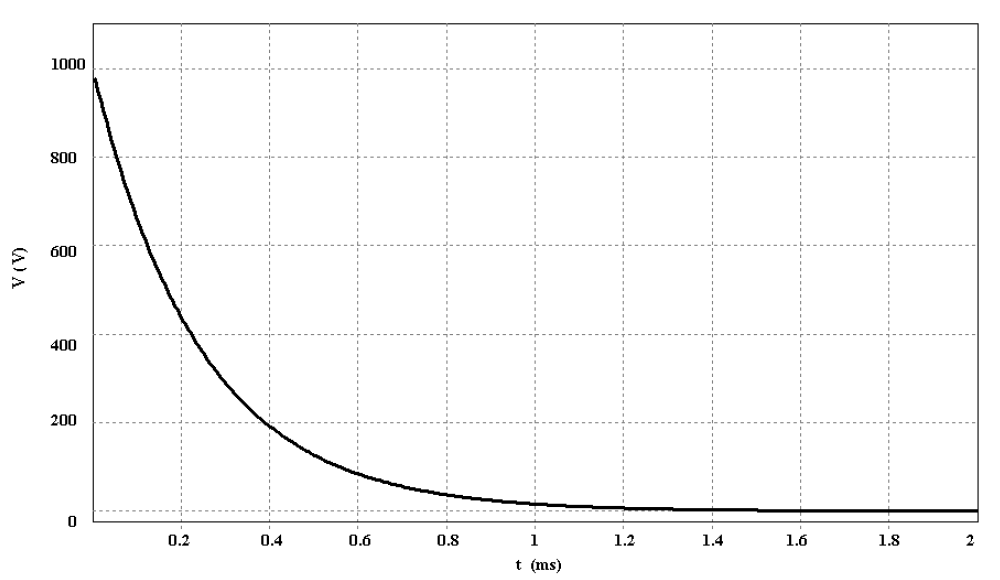
\includegraphics[width=16cm]{figuras/tensaoimpedanciahumana}}
		}
			\Fonte{elaborada pelo autor.}
			
\end{figure}

Texto texto texto texto texto texto texto texto texto texto texto texto texto texto texto texto texto texto texto texto texto texto texto texto texto texto texto texto texto texto texto texto texto texto texto texto texto texto texto texto texto texto texto texto texto texto texto texto texto texto texto texto texto texto texto texto texto texto texto texto texto texto texto texto texto texto texto texto texto.

\begin{figure}[h!]
	\captionsetup{width=16cm}
	\Caption{\label{fig-grafico-1}Produção anual das dissertações de mestrado e teses de doutorado entre os anos de 1990 e 2008}		
	\IBGEtab{}{
		\fbox{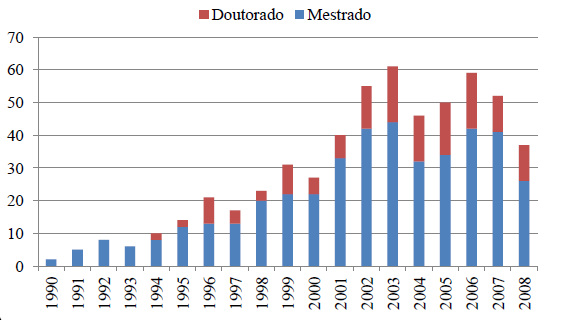
\includegraphics[width=16cm]{figuras/figura-3}}
	}{
	\Fonte{elaborada pelo autor.}
}
\end{figure}

Texto texto texto texto texto texto texto texto texto texto texto texto texto texto.

Texto texto texto texto texto texto texto texto texto texto texto texto texto texto texto texto texto texto texto texto texto texto texto texto texto texto texto texto texto texto texto texto texto texto texto texto texto texto texto texto texto texto texto texto texto texto texto texto texto texto texto texto texto texto texto texto texto texto texto texto texto texto texto texto texto texto texto texto texto.

\section{Resultados do Experimento B}
\label{sec:resultados-do-experimento-b}

Referenciando a \autoref{tab:notas}. Texto texto texto texto texto texto texto texto texto texto texto texto texto texto texto texto texto texto texto texto texto texto texto texto texto texto texto texto texto texto texto texto.

\begin{table}[!ht]	
	%\centering
	\captionsetup{width=11.3cm}%ATENÇÃO: Ajuste a largura do título
	\Caption{\label{tab:notas} Notas dos participantes nas avaliações A, B e C}	
	\IBGEtab{}{
		\begin{tabular}{crrr}
			\toprule
			Identificação dos participantes & Avaliação A & Avaliação B &                        Avaliação C \\
			\midrule \midrule
			Participante 1 & 7 & 9 & 10\\
			Participante 2 & 8 & 2 & 1\\
			Participante 3 & 5 & 10 & 6 \\
			Participante 4 & 3 & 1 & 4\\
			Participante 5 & 2 & 4 & 1\\
			Participante 6 & 0 & 7 & 2\\
			\bottomrule
		\end{tabular}
	}{
	\Fonte{elaborada pelo autor.}
}
\end{table}

Texto texto texto texto texto texto texto texto texto texto texto texto texto texto texto texto texto texto texto texto texto texto texto texto texto texto texto texto texto texto texto texto texto texto texto texto texto texto texto texto texto texto texto texto texto texto texto texto texto texto texto texto texto texto texto texto texto texto texto texto texto texto texto texto texto texto texto texto texto.Texto texto texto texto texto texto texto texto texto texto texto texto texto texto texto texto texto texto texto texto texto texto texto texto texto texto texto texto texto texto texto texto texto texto texto texto texto texto texto texto texto.

Texto texto texto texto texto texto texto texto texto texto texto texto texto texto texto texto texto texto texto texto texto texto texto texto texto texto texto texto texto texto texto texto texto texto texto texto texto texto texto texto texto texto texto texto texto texto texto texto.Texto texto texto texto texto texto texto texto texto texto texto texto texto texto texto texto texto texto texto texto texto.

Referenciando a \autoref{tab:notas}. Texto texto texto texto texto texto texto texto texto texto texto texto texto texto texto texto texto texto texto texto texto texto texto texto texto texto texto texto texto texto texto texto texto texto texto texto texto texto texto texto texto texto texto texto texto texto texto texto texto texto texto texto texto texto texto texto texto texto texto texto texto texto texto texto texto texto texto.
	%\chapter{Conclusões e Trabalhos Futuros}
\label{chap:conclusoes-e-trabalhos-futuros}

Parte final do texto na qual se apresentam as conclusões apoiadas no desenvolvimento do assunto. É a recapitulação sintética dos resultados obtidos. Pode apresentar recomendações e sugestões para pesquisas futuras.

%\label{sec:contribuicoes-do-trabalho}



%\label{sec:limitacoes}








	
	%Elementos pós-textuais	
	\bibliography{3-pos-textuais/referencias}
%	\imprimirglossario %	
	%\imprimirapendices
		% Adicione aqui os apendices do seu trabalho
		%\apendice{EXEMPLO DE APÊNDICE}
\label{ap:A}

Um apêndice é um documento elaborado pelo autor, diferentemente do anexo. Geralmente, se coloca como apêndice, questionários, códigos de programação, tabelas que tomariam muito espaço no meio do trabalho.
		%\apendice{ Questionário utilizado para}
\label{ap:B}

\begin{questao}
	\item Esta é a primeira questão com alguns itens:
		\begin{enumerate}
			\item Este é o primeiro item
			\item Segundo item
		\end{enumerate}
	\item Esta é a segunda questão:
		\begin{enumerate}
			\item Este é o primeiro item
			\item Segundo item
		\end{enumerate}
	\item Lorem ipsum dolor sit amet, consectetur adipiscing elit. Nunc dictum sed tortor nec viverra. consectetur adipiscing elit. Nunc dictum sed tortor nec viverra.
		\begin{enumerate}
			\item consectetur
			\item adipiscing
			\item Nunc
			\item dictum
		\end{enumerate}
\end{questao}

		%\apendice{ Códigos-fontes utilizados para}
\label{ap:C}

\lstinputlisting[language=C++,caption={Hello World em C++}]{figuras/main.cpp}


\begin{lstlisting}[language=Java,caption={Hello World em Java}]
public class HelloWorld {
	public static void main(String[] args) {
		System.out.println("Hello World!");
	}
}
\end{lstlisting}


		
		%\imprimiranexos
		% Adicione aqui os anexos do seu trabalho
		%\anexo{ Exemplo de um anexo}
\label{an:ex_anexo_a}

Um anexo é um documento que não foi elaborado pelo autor, ou seja, o autor apenas anexa. Anexos podem ser tabelas, mapas, diagramas, \textit{datasheets}, manuais e etc. 




		%\anexo{ Exemplo de um anexo em PDF}
\label{an:ex_anexo_b}

O autor pode anexar um \gls{PDF}, traduzido como formato portátil de documento. Veja o código fonte utilizado para anexar o arquivo ``Sikasil.pdf'' que foi colocado dentro da pasta ``anexos'' que por sua vez está dentro da pasta ``elementos-pos-textuais''. Tenha muita atenção na hora de especificar o local do arquivo. Recomenda-se não utilizar caracteres especiais para nomear pastas e, principalmente, arquivos. 

Pode-se fazer uma descrição sucinta do arquivo anexado.

%Comando para incluir um arquivo em PDF:
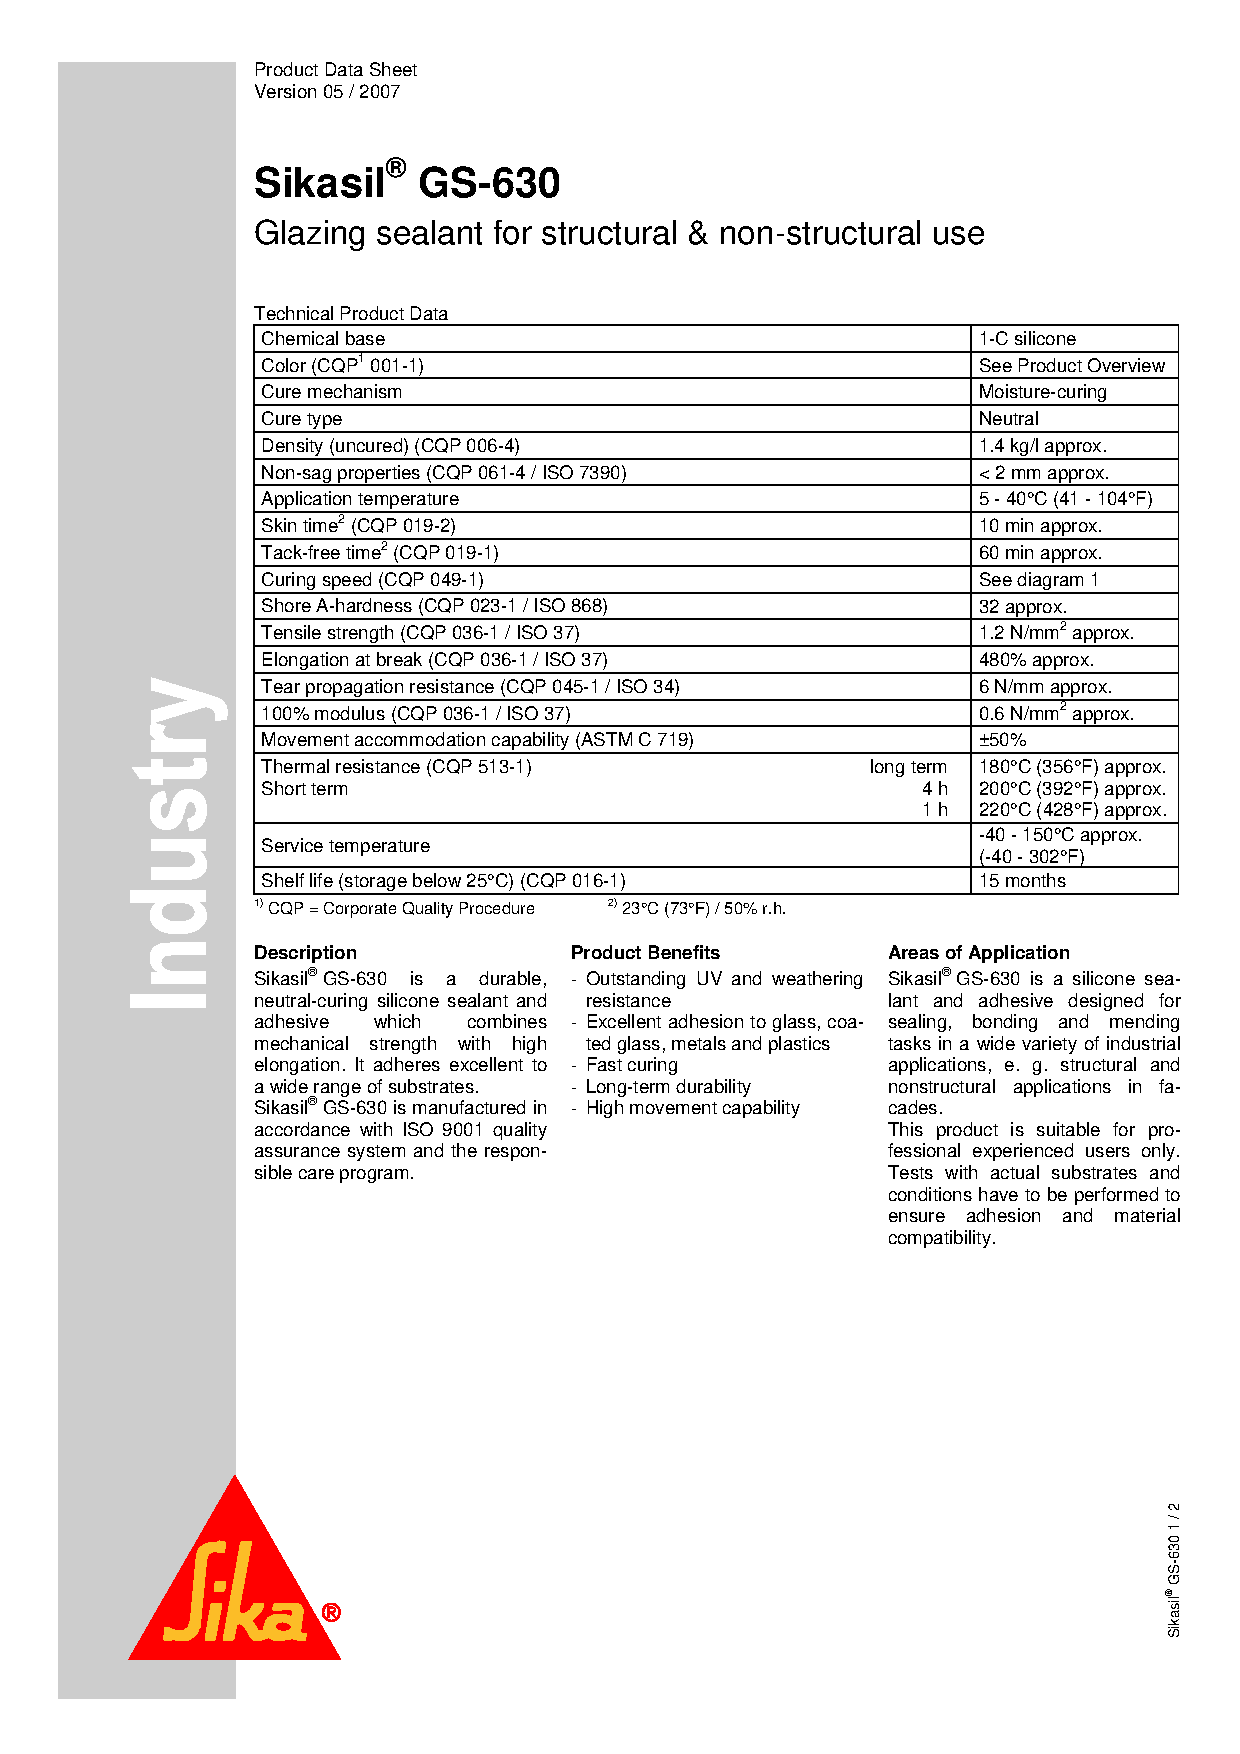
\includepdf[pages={-}]{3-pos-textuais/anexos/Sikasil.pdf}

		
    %\imprimirindice
    
	

\end{document}